\documentclass{article}
\usepackage[english]{babel}
\usepackage[utf8]{inputenc}
\usepackage{fancyhdr}
\usepackage{geometry}
\usepackage{enumitem}
\usepackage{amsmath}
\usepackage{graphicx}
\usepackage{tcolorbox}
\usepackage{amssymb}
\usepackage[thinc]{esdiff}
\usepackage{float}

\geometry{letterpaper, portrait, margin=1in}
\graphicspath{ {images/} }
\pagestyle{fancy}
\fancyhf{}
\lhead{Keerthik Muruganandam}
\rhead{Yadavalli Homework 2}

\begin{document}

\begin{enumerate}[label=\textbf{(2.\arabic*)}] %%%%%%%%%%%%%%%%%%%%%%%%%%%%%%%%%%%%%%%%%%%%%%%%%%%%%%%%%%%%%%

\item Use Part 1 of the FTC to calculate the derivative of $f(x)=\displaystyle{ \int_{x^2}^{\cos(x)}\!\ln\left(1+v^4\right)\,dv }$.
\newline
The FTC works with the integral with bounds $(0,x)$. Since the upper bound of the original integral was $\cos(x)$, we can take the integral from 0 to $\cos(x)$ and subtract the area from 0 to $x^2$ to get just the area from $x^2$ to $\cos(x)$. Thus we can split the integral into two parts with a constant as a bound.
\[\int_0^{\cos(x)}\!\ln\left(1+v^4\right)\,dv-\int_0^{x^2}\!\ln\left(1+v^4\right)\,dv\]
Using the Evaluation Theorem we can see that the derivative should look like this:

\begin{align*}
\diff{}{x}\left(\int_0^{\cos(x)}\!\ln\left(1+v^4\right)\,dv-\int_0^{x^2}\!\ln\left(1+v^4\right)\,dv\right) &= \diff{}{x}\left(V(\cos(x))-V(0)-V\left(x^2\right)+V(0)\right) \\
&=\diff{}{x}\left(V(\cos(x))-V\left(x^2\right)\right) \\
&=v(\cos(x))\diff{}{x}\cos(x)-v\left(x^2\right)\diff{}{x}x^2 \\
&= -v(\cos(x))\sin(x)-2v\left(x^2\right)
\end{align*}

Now that we have shown how to compute the derivative of the integrals, we can simplify to get
\[-\ln\left(1+\cos^4(x)\right)\sin(x)-2\ln\left(1+x^16\right)\]
So we know that the derivative of $f(x)$ is $-\left(\ln\left(1+\cos^4(x)\right)\sin(x)+2\ln\left(1+x^16\right)\right)$ \\
\newline

\begin{center}
Next Problem on Page 2.$ \rightarrow$
\end{center}

\newpage %%%%%%%%%%%%%%%%%%%%%%%%%%%%%%%%%%%%%%%%%%%%%%%%%%%%%%%%%%%%%%%%%%%%%%%%%%%%%%%

\item Let $g(x)= \displaystyle{ \int_0^x\! f(x) \, dt }$, where $f(x)$ is the function whose graph is shown below.

\begin{enumerate}[label=(\alph*)]
\item Evaluate $g(x)$ for $x=0,1,2,3,4,5,6$
\item On what interval is $g(x)$ increasing?
\item Sketch a graph of $y=g(x)$
\item Use the graph in (c) to sketch the graph of $g^\prime(x)$. How does this sketch compare with the graph of $f$.
\end{enumerate}

\begin{figure}[H]
\centering
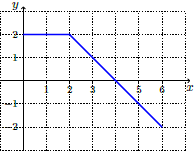
\includegraphics{twopointtwo}
\end{figure}

\begin{enumerate}[label=(\alph*)]
\item We can just use the ''counting squares'' method to calculate these values. If we do, we get the values
\[g(0)=0, g(1)=2, g(2)=4, g(3)=5.5, g(4)=6, g(5)=5.5, g(6)=4\]
\item To find the interval on which $g(x)$ is increasing we can look at our previous calculations. From those values we can see that from $x=0$ to $x=4$, the values were increasing. To back this up with calculus, we can say that the values for $f(x)$ are above zero until $x=4$, so when the function passes below the x-axis, the values start becoming smaller because negative area is being added to the previous sums. \\
Thus the function is increasing on the interval $(0,4)$.
\item See graph below.

\begin{figure}[H]
\centering
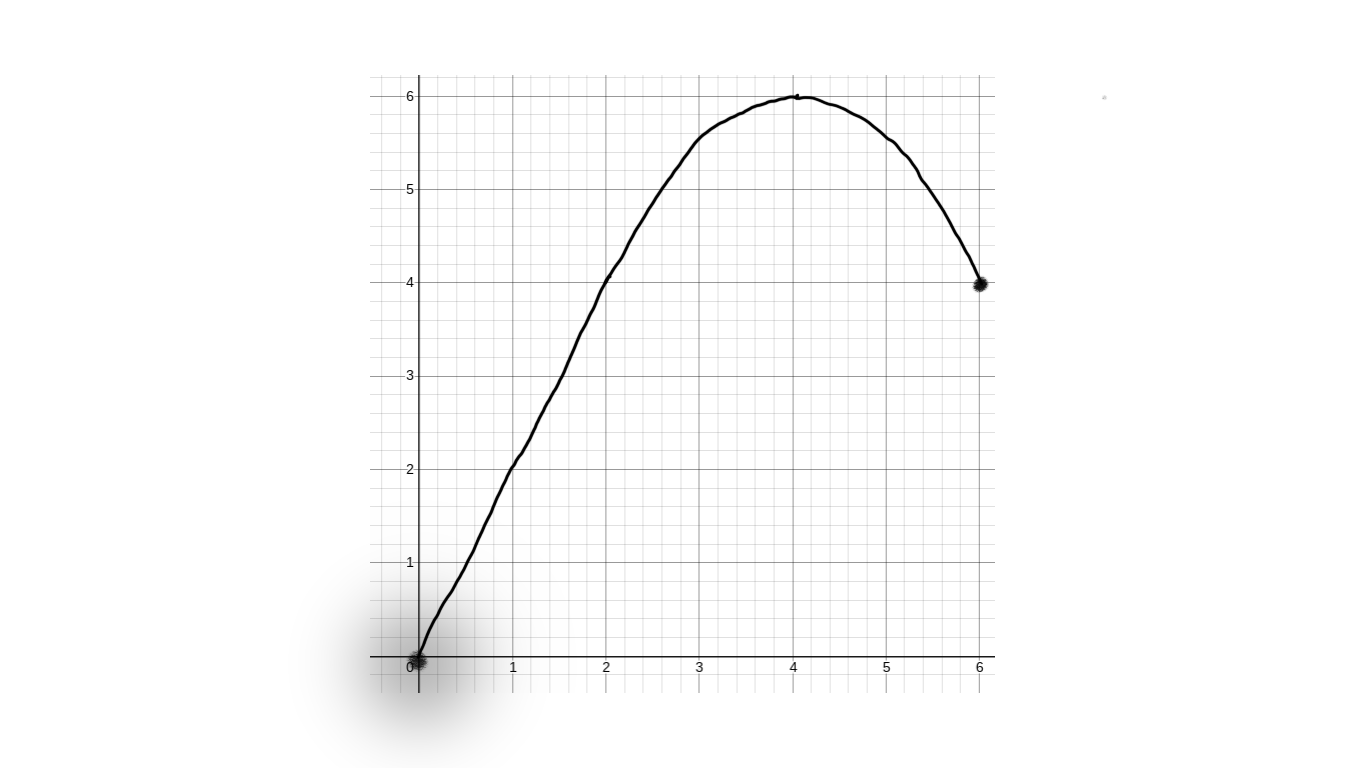
\includegraphics[scale=.10]{twosies}
\end{figure}

\item If we sketch the derivative of $g(x)$, we get the function

\begin{figure}[H]
\centering
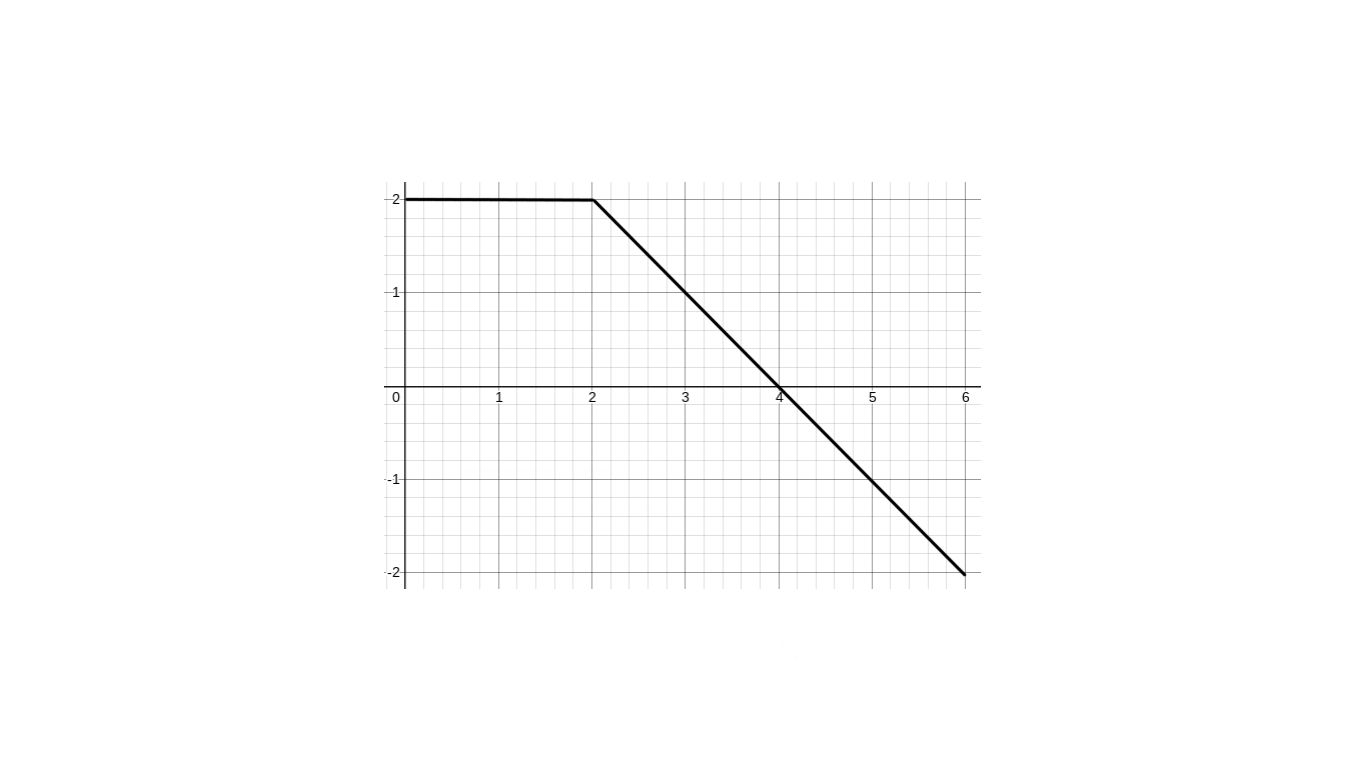
\includegraphics[scale=.15]{threesies}
\end{figure}

The graph of the derivative is the same as $f(x)$ in the original integral! We can see that this is true because of the FTC. We have just shown the FTC geographically.
\end{enumerate}

\newpage %%%%%%%%%%%%%%%%%%%%%%%%%%%%%%%%%%%%%%%%%%%%%%%%%%%%%%%%%%%%%%%%%%%%%%%%%%%%%%%

\item Let $g(x)=\displaystyle{\int_0^x\!f(t)\,dt}$, where $f$ is the graph below. Answer the following questions:

\begin{enumerate}[label=(\alph*)]
\item At what values of $g$ do local minimum and maximum values of $g$ occur?
\item Where does $g$ attain its absolute maximum value?
\item On what intervals is $g$ concave downwards?
\item Sketch the graph of $g$.
\end{enumerate}

\begin{figure}[H]
\centering
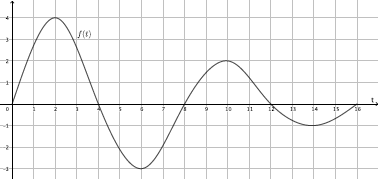
\includegraphics{twopointthree}
\end{figure}

\begin{enumerate}[label=(\alph*)]
\item We can see that the local minimums and maximums are at the x-intercepts of $f$ because that's where the function peaks before area of teh opposite sign starts being added, either reducing or increasing the area that was previously only increasing/decreasing. If we continue this train of though, we see that the x-intercept right after a section of positive area is a max and one right after some negative area is a min. \\
Thus the local minimums are $0, 8, 16$ and the local maximums are 4 and 12.
\item The problem states that we can assume that the absolute values of the area for each hump is decreasing from left to right. Thus we can conclude that the area of each hump doesn't completely counteract the previous hump. Therefore, the area lost from $(0,4)$ by $(4, 8)$ is never completely recovered. Now we conclude that the area reaches it's absolute maximum at $x=4$.
\item $g(x)$ is concave down on the intervals $(2,6)$ and $(10,14)$. We can use the fact that $f(x)=g^\prime(x)$ due to the FTC and when $g^\prime(x)$ is increasing, $g^{\prime\prime}(x)$ is above zero to imply that whenever $f(x)$ is decreasing, the function is concave down. Thus we get our intervals $(2,6)$ and $(10,14)$.
\item Graph Below
\begin{figure}[H]
\centering
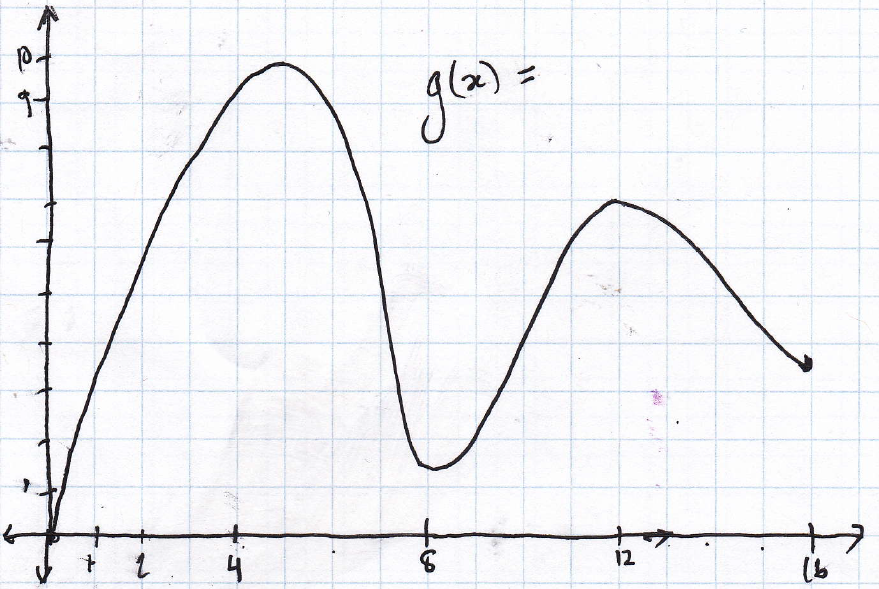
\includegraphics[scale=.25]{foursies}
\end{figure}
\end{enumerate}
\newpage %%%%%%%%%%%%%%%%%%%%%%%%%%%%%%%%%%%%%%%%%%%%%%%%%%%%%%%%%%%%%%%%%%%%%%%%%%%%%%%

\item \textbf{Professional Problem:} Let
\[f(x)= \begin{cases}
0, \text{        if } x<0 \\
2x, \text{       if } 0\le x\le1 \\
4-2x, \text{       if } 1<x\le2 \\
0, \text{       if } x>2
\end{cases}\]
And let $g(x)=\displaystyle{ \int_0^x\!f(t)\,dt }$. Find an explicit formula for $g(x)$ which doesn't involve integrals. \\
\newline
To start, let's visualize the function $f(x)$. See the graph below
\begin{figure}[H]
\centering
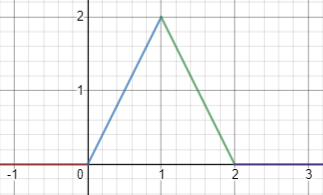
\includegraphics[scale=.5]{twopointfour}
\end{figure}
Thus we can see that $g(x)$ will not yield a positive nonzero integer unless $x>0$. \\ 
Therefore, in the pievewise function we are constructing, we can keep that $g(x)=0, \text{ if } x<0$. \\
Now let's look at x values within the range of $(0,1]$.  We can clearly see that the area will be the area underneath the line $2x$. Thus, we can use the Evaluation Theorem to find an integral-less version of the function. The expression looks like
\[\int_0^x\!2t\,dt=2t{|}_0^x=F(x)-F(0)=x^2-0^2=x^2\]
Now we can use the equation $x^2$ for the integral on the bound (0,1]. \\
 Moving on, we must tackle the interval $(1,2]$. Again looking at the graph of $f(x)$ the function on that interval is $-2x+4$. We can use the same process as we did for the prior integral and the output looks like
 \[\int_0^x\!(4-2t)\,dt=(4-2t)|_0^x=F(x)-F(0)=4x-x^2-4(0)-0^2=4x-x^2\]
 We can see that using the simple process of using the Evaluation Theorem and antiderivatives we have eliminated all integrals from $g(x)$ because the integral of 0 is 0 for when $x>2$. \\
 In conclusion, the final piecewise function looks like
 \[g(x)= \begin{cases}
 0, \text{ if } x<0 \\
 x^2,\text{ if } 0\le x\le1 \\
 4x-x^2,\text{ if }1<x\le2 \\
 0, { if } x>2
 \end{cases} \]
 Now, if we graph this equation, we get the graph
 \begin{figure}[H]
 \centering
 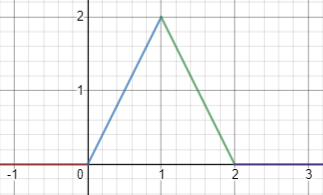
\includegraphics[scale=.5]{fivesies}
 \end{figure}
 Thus, we have found an explicit formula for $g(x)$ not involving any integrals and graphed it.
\end{enumerate}%%%%%%%%%%%%%%%%%%%%%%%%%%%%%%%%%%%%%%%%%%%%%%%%%%%%%%%%%%%%%%%%%%%%%%%%%%%%


\end{document}